\newpage
\section{Modellierung} % (fold)
\label{sec:modellierung}

\subsection{Ereignisgesteuerte Prozessketten} % (fold)
\label{sub:ereignisgesteuerte_prozessketten}

Aus der Aufgabenbeschreibung ergeben sich die in Abbildung~\ref{fig:epk} dargestellten \ac{EPK} für Erzeuger und Verbraucher. Hierbei ist zu erkennen, dass sich die Prozesse bei identischem Ablaufschema lediglich in den  durchgeführten Prüfungen und Operationen unterscheiden. Hierdurch liegt es nahe, dass die Ablaufsteuerung im objektorientierten Entwurf in einer abstrakten Basisklasse modelliert wird, und nur die unterschiedlichen Handlungen in den jeweiligen spezialisierten Ableitungen konkretisiert werden.

\begin{figure}[H]
\begin{center}
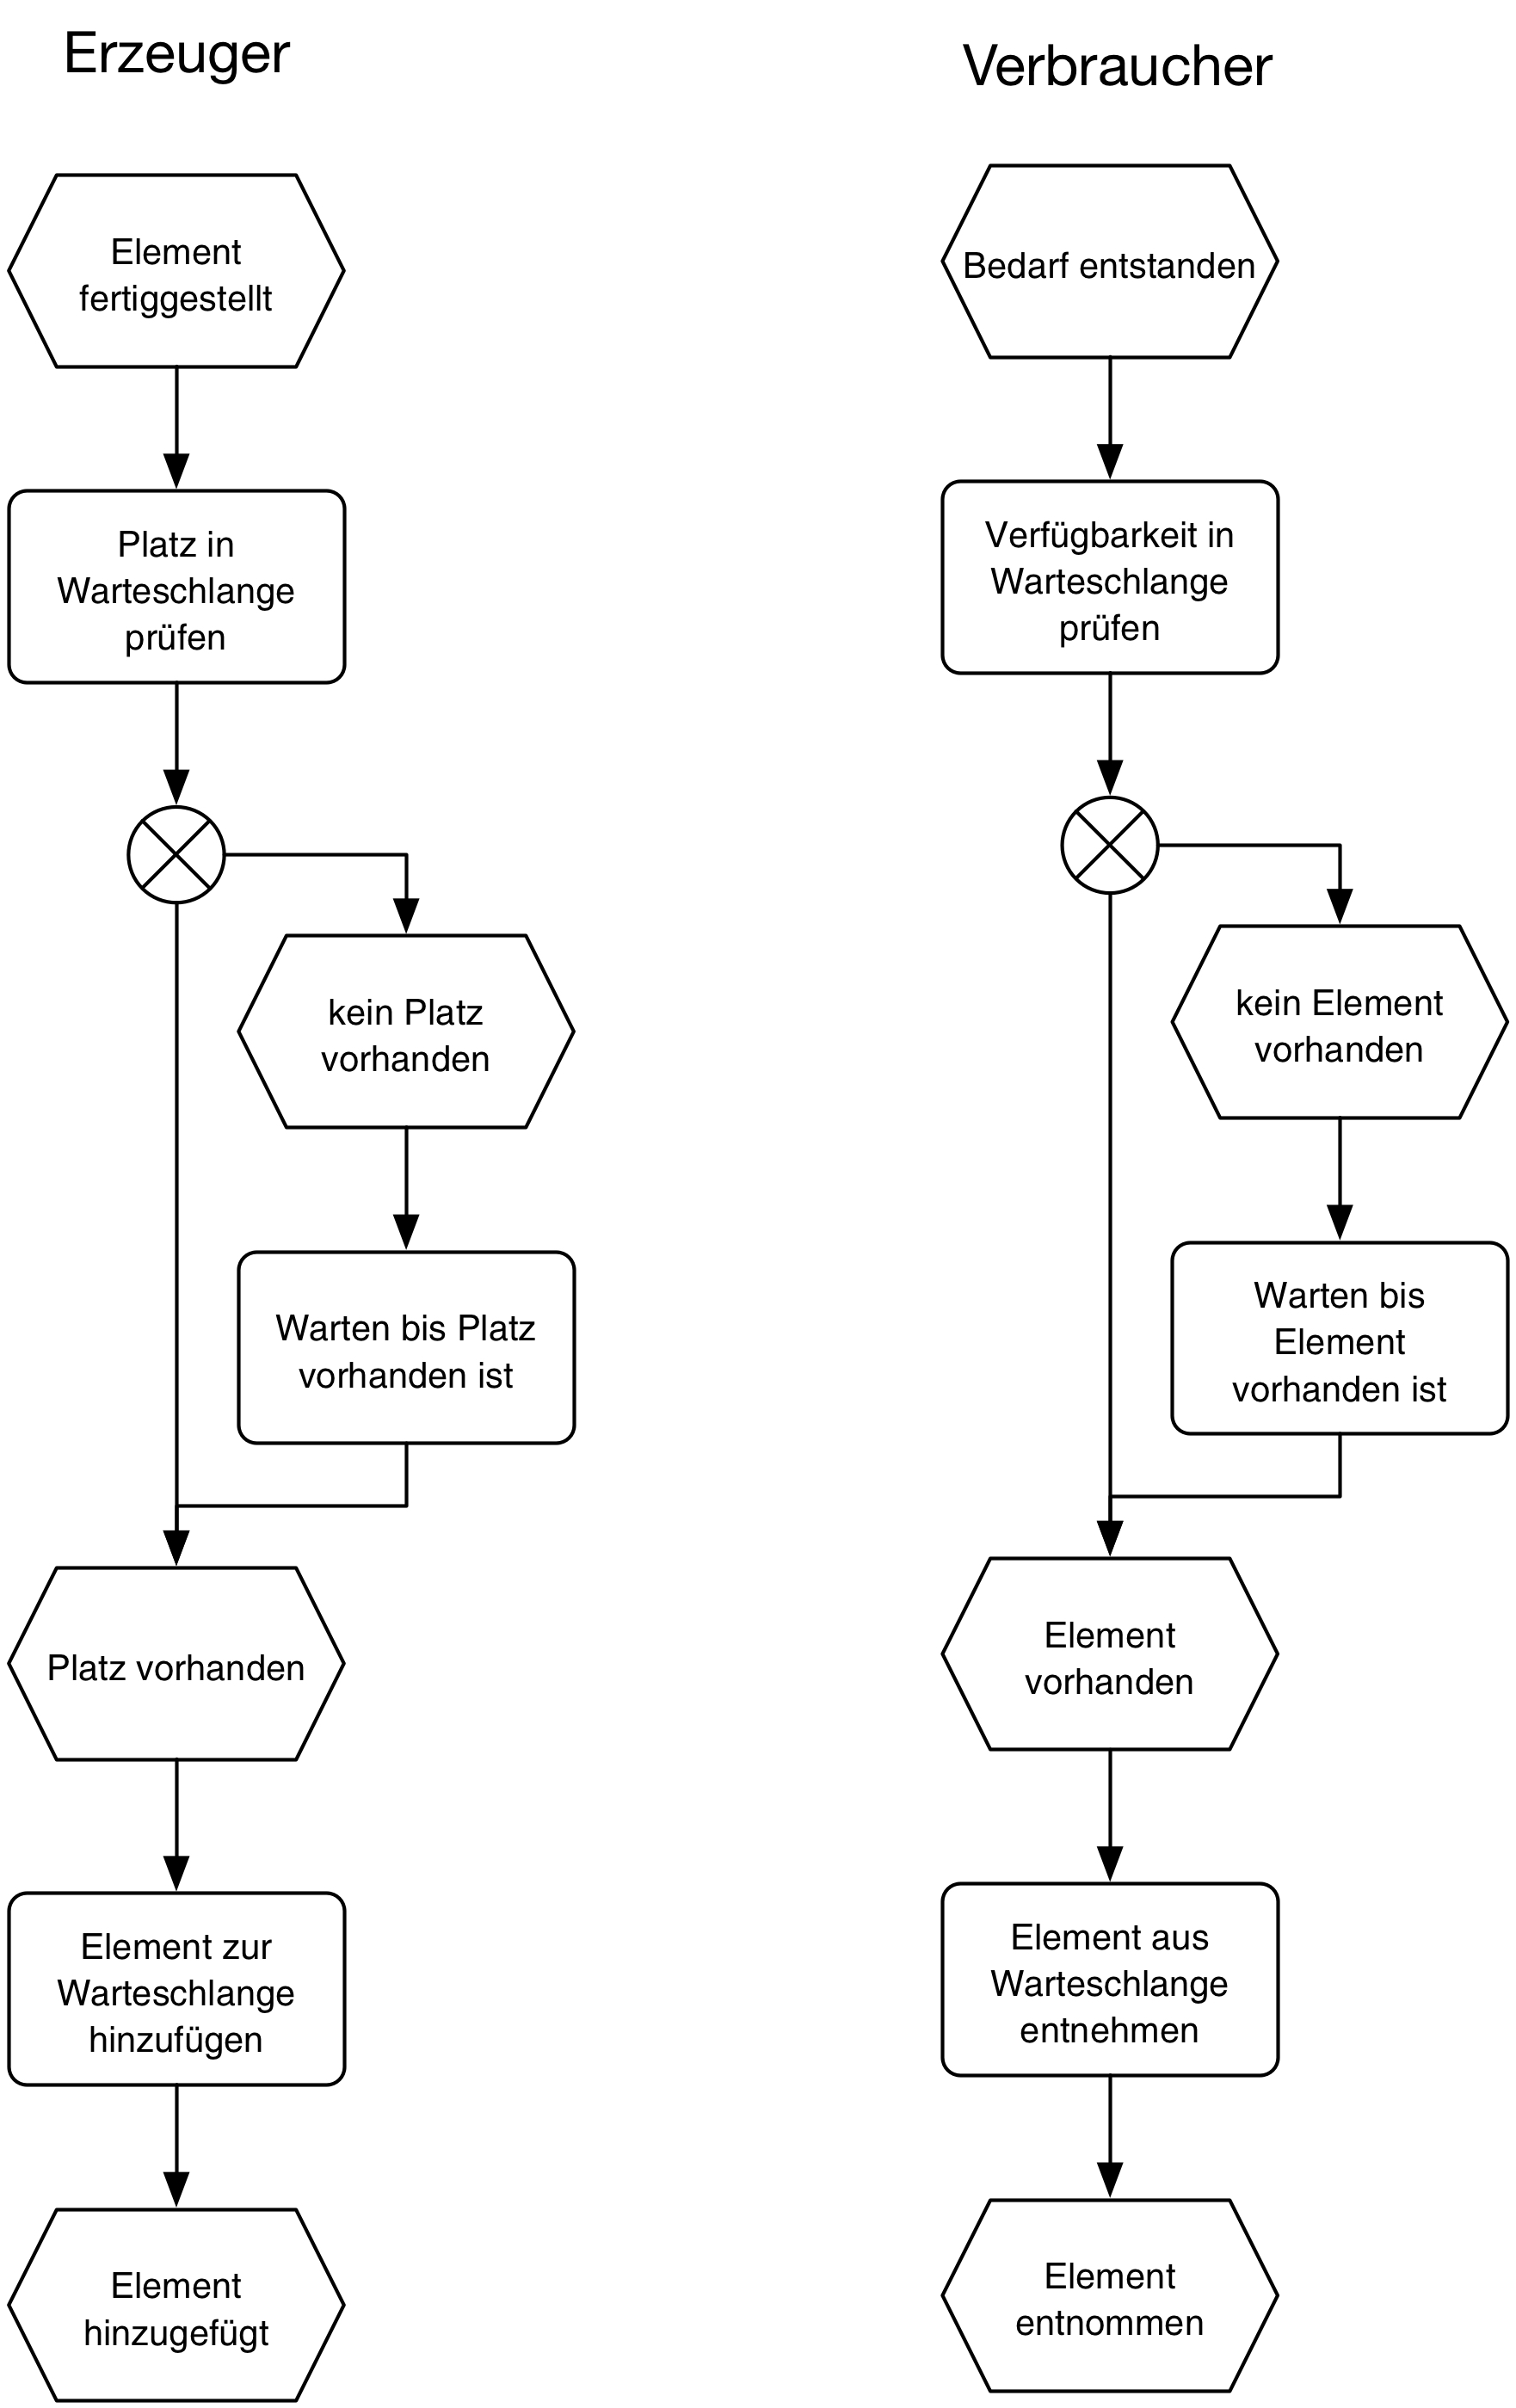
\includegraphics[width=.5\textwidth]{Erzeuger-Verbraucher-EPK.jpg}
\caption{Ereignisgesteuerte Prozessketten}
\label{fig:epk}
\end{center}
\end{figure}

% subsection ereignisgesteuerte_prozessketten (end)

\subsection{UML–Diagramm} % (fold)

In Abbildung~\ref{fig:epk} sind die zur Implementierung benötigten Klassen sowie deren Beziehungen untereinander als UML–Diagramm dargestellt. Die entsprechenden Erläuterungen finden sich in Kapitel~\myref{sec:implementierung}.

\label{sub:uml_diagramm}
\begin{figure}[H]
\begin{center}
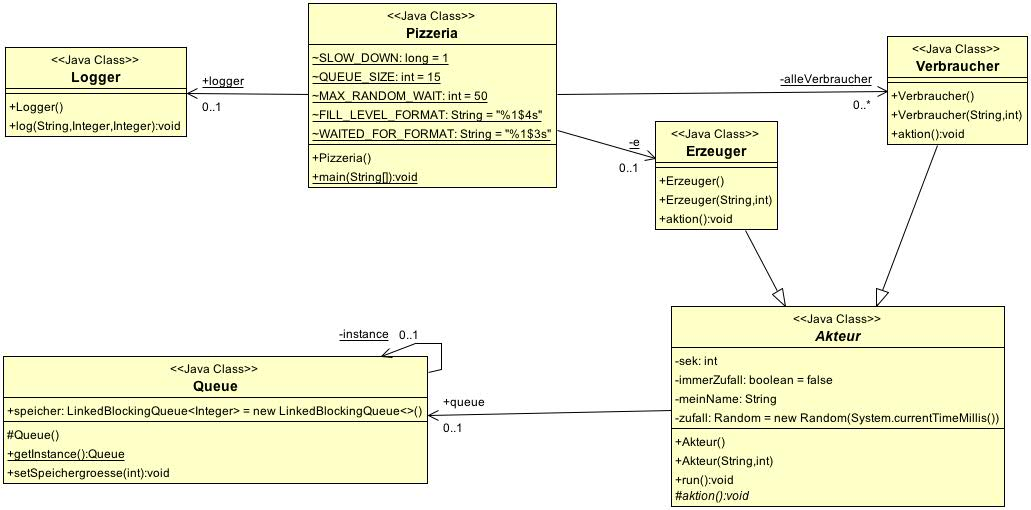
\includegraphics[width=\textwidth]{UML.jpg}
\caption{UML–Diagramm}
\label{fig:epk}
\end{center}
\end{figure}
% subsection uml_diagramm (end)

% section modellierung (end)

\section{Implementierung} % (fold)
\label{sec:implementierung}

\subsection{Klasse: Akteur} % (fold)
\label{sub:klasse_akteur}
In der der abstrakten Klasse \code{Akteur} werden die Eigenschaften und Methoden zusammengefasst, die den Klassen \code{Erzeuger} und \code{Verbraucher} gemeinsam sind. Dazu gehören die Angaben zur Wartezeit \code{sek} bzw. \code{immerZufall} sowie die Bezeichnung \code{meinName}, die bei der Ausgabe dazu dienen kann, die Akteure zu unterscheiden. Diese Variablen werden von den Konstruktoren beim Erzeugen der Objekte befüllt. Des weiteren wird ein Generator für Pseude–Zufallszahlen sowie eine Referenz auf die Warteschlange benötigt.

In der Methode \code{run()}, die beim Starten des Threads aufgerufen wird, wird zunächst wie gefordert der Name und der Füllstand der Queue, ergänzt mit der Wartezeit ausgegeben. Anschließend wird die abstrakte Methode \code{aktion()} aufgerufen, welche die spezifischen Aktionen der abzuleitenden Klassen ausführt. Abschließend wird durch Aufruf der Methode \code{sleep()} der Elternklasse \code{Thread} die vorgegebene oder zufällig bestimmte Zeit gewartet.

Die Klasse \code{Akteur} implementiert keinen Zugriff auf die Queue und betritt somit keinen kritischen Abschnitt.
% subsection klasse_akteur (end)

\subsection{Klasse: Erzeuger} % (fold)
\label{sub:klasse_erzeuger}
Die von \code{Akteur} abgeleitete Klasse \code{Erzeuger} implementiert lediglich die Methode \code{aktion()}. Hierzu muss der kritische Abschnitt betreten werden. Hierin muss geprüft werden, ob Platz in der Queue vorhanden ist. Falls nicht, muss gewartet werden, bis dies der Fall ist. Wenn Platz vohanden ist, wird das produzierte Element\footnote{Hierbei handelt es sich in der Simulation um den Integerwert 1} in der Queue abgelegt. Anschließend wird der kritische Abschnitt wieder verlassen.

Diese Vorgehensweise entspricht der Implementierung der \code{put() } der Klasse \code{LinkedBlockingQueue}, welche indirekt über die Klasse \code{Queue} aufgerufen wird.\footnote{vgl. \cite{javadoc:lbqsourceput}}

Wie im Abschnitt~\myref{sub:kritische_abschnitte} ausgeführt, sind das Hinzufügen und das Entnehmen von Elementen bei \ac{FIFO} Warteschlangen getrennte kritische Abschnitte. Somit kann das Warten im Falle einer vollen Warteschlange durchgeführt werden, ohne eine Deadlock–Situation herbeizuführen.
% subsection klasse_erzeuger (end)

\subsection{Klasse: Verbraucher} % (fold)
\label{sub:klasse_verbraucher}
Die von \code{Akteur} abgeleitete Klasse \code{Verbraucher} implementiert lediglich die Methode \code{aktion()}. Hierzu muss der kritische Abschnitt betreten werden. Hierin muss geprüft werden, ob mindestens ein Element in der Queue vorhanden ist. Falls nicht, muss gewartet werden, bis dies der Fall ist. Wenn ein Element vohanden ist, wird das älteste entnommen. Anschließend wird der kritische Abschnitt wieder verlassen.

Diese Vorgehensweise entspricht der Implementierung der \code{take()} der Klasse \code{LinkedBlockingQueue} welche indirekt über die Klasse \code{Queue} aufgerufen wird.\footnote{vgl. \cite{javadoc:lbqsource}} 
% subsection klasse_verbraucher (end)

\subsection{Sonstige Programmmerkmale} % (fold)
\label{sub:sonstige_programmmerkmale}
Die Klasse \code{Queue} realisiert das Singleton–Entwurfsmuster, um ein Element der Klasse \code{LinkedBlockingQueue} der gewünschten Größe allen beteiligten Objekten und damit allen Threads zugänglich zu machen.\footnote{vgl. \cite{gof}, Seite 127ff}

Die Klasse \code{Logger} übernimmt die geforderte Ausgabe von „E“ bzw. „V” gefolgt von der Angabe der Zahl der momentan in der Warteschlange vorhandenen Elementen. Ergänzt werden diese Angaben von der Wartezeit\footnote{Hierbei ist die Wartezeit innerhalb des kritischen Abschnitts nicht berücksichtigt} und der dem Verbraucher zugewiesenen laufenden Nummer. Durch die Ausgabe des kompletten, zuvor zusammengesetzten Ausgabestrings in einem einzigen Aufruf von \code{System.out.println()} wird hier der konkurrierende Zugriff auf die gemeinsame Resource der Bildschirmausgabe threadischer geregelt.\footnote{siehe auch Abschnitt~\myref{sub:realisierung_mit_linkedblockingqueue}}

Die Klasse Pizzeria stellt das Gerüst der Anwendung dar. Hierin werden neben einigen Konstanten auch die benötigten Obkekte der Klassen \code{Logger} und \code{Erzeuger} sowie eine \code{ArrayList} für die nach dem Programmstart zu bestimmende Anzahl der Verbraucher definiert. Die Wartezeiten für die Verbraucher und den Erzeuger werden abgefragt und die Threads erzeugt und gestartet. Hierbei wird auch die vom Nutzer gewählte Konfiguration erfasst und zur Dokumentation in den Ausgabestrom geschrieben. Anschließend werden alle weiteren Schritte des Programms in den Threads ausgeführt. 
% subsection sonstige_programmmerkmale (end)
% section implementierung (end)

\section{Laufzeitbetrachtungen} % (fold)
\label{sec:laufzeitbetrachtungen}

\subsection{Generelle Beobachtungen} % (fold)
\label{sub:generelle_beobachtungen}
Die erstellte Anwendung wurde in unterschiedlichen Konfigurationen ausgeführt. Ein der Aufgabenstellung entsprechender Programmlauf ist z.B. in der Logdatei \code{e0v0.0.0.txt} dokumentiert. Hier wurden ein Erzeuger–Thread und drei Verbraucher–Threads ausgeführt, deren Wartezeiten zufällig bestimmt wurden. In diesem Programmlauf zeigen sich einige interessante Abschnitte, welche im folgenden Abschnitten auch anhand von weiteren Programmläufen näher betrachtet werden.

Besonderes Augenmerk soll auf den Füllständen der Warteschlange liegen. Wie oft trifft ein Verbraucher auf eine leere Warteschlange\footnote{z.B. in den meisten Fällen bei \code{e0v0.0.0.txt}}, wie oft ein Erzeuger auf eine volle Warteschlange\footnote{z.B. in Zeile 2589 von \code{e0v0.txt}}. Dies sind die Situationen, in denen die Programmausführung ins Stocken gerät. Ebenfalls wird die Anzahl der Situationen ermittelt, in denen weder Verbraucher noch Erzeuger warten mussten. Diese Situationen sind wohl in den meisten Fällen als Idealzustand anzusehen.

\begin{landscape}
\begin{footnotesize}
\begin{table}[H]
\begin{center}
\begin{tabular}{| p{3cm} | p{3cm} || r | r | r | r r | r r | r r |}  \hline                       
  \textbf{Erzeuger}	& \textbf{Verbraucher}  & \textbf{….put()} & \textbf{….take()} & \textbf{Gesamt} & \multicolumn{2}{|l|}{\textbf{E wartet}} & \multicolumn{2}{|l|}{\textbf{V wartet}} & \multicolumn{2}{|l|}{\textbf{ohne Warten}}  \\ \hline 
zufällig 		& 3, zufällig & 11.612 			 & 11.614 			 & 23.226 		   & 0 		 & 0,00\% 						 & 11.383  & 98,01\% 					   & 11.843		&	50,99\%	\\ \hline
zufällig 		& 1, zufällig & 11.593		     & 11.592 			 & 23.185 		   & 228 	 & 1,97\% 						 & 465     &  4,01\% 					   & 22.492		&	97,01\%	\\ \hline
1 ZE 			& 6, zufällig & 70.442 	 	     & 70.432 			 & 140.874 		   & 15268 	 & 21,67\% 						 & 1       &  <0,01\% 					   & 125.605	&  89,16\%	\\ \hline
1 ZE 			& 7, zufällig & 82.070 	 		 & 82.054 			 & 164.124 		   & 2912    & 3,55\% 						 & 328     & 0,40\% 					   & 160.884		&	98,03\%	\\ \hline
1 ZE 			& 8, zufällig & 84.068 	 		 & 84.069 			 & 168.137 		   & 0 	 & 0,00\% 						 & 48.162  & 57,29\% 					   & 119.975	&	71,36\%	\\ \hline
1 ZE & 8, mit 5, 7, 11, 13, 17, 19, 23 und 42 ZE & 60.680 & 60.660	 & 121.340 		   & 23869 		 & 39,34\% 						 & 5  & 0,01\% 					   & 97.466		&	80,32\%	\\ \hline
\end{tabular}
\caption{Eckdaten einiger Simulationsläufe}
\label{tab:ergebnisse}
\end{center}
\end{table}
\textbf{Legende:} \textbf{Erzeuger}: Wartezeit des Erzeugers in \ac{ZE}; \textbf{Verbraucher:} Anzahl und Wartezeiten der Verbraucher in \ac{ZE}; \textbf{….put():} Anzahl der Elemente, die der Warteschlange hinzugefügt wurden; \textbf{….take():} Anzahl der Elemente, die der Warteschlange entnommen wurden; \textbf{E wartet:} Wie oft musste der Erzeuger auf Platz in der Warteschlange warten. Die Prozentangabe bezieht sich auf die in Spalte „….put()“ angegebene Zahl ; \textbf{V wartet:} Wie oft mussten Verbraucher auf Elemente in der Warteschlange warten. Die Prozentangabe bezieht sich auf die in Spalte „….take()“ angegebene Zahl; \textbf{Gesamt:} Wie oft konnten die Operationen an der Warteschlange ohne unfreiwillige Wartezeit durchgeführt werden. Die Prozentangabe bezieht sich auf die in Spalte „Gesamt“ angegebene Zahl; Die Logdateien der Simulationsläufe sind der elektronischen Form dieser Arbeit beigefügt.
\end{footnotesize}
\end{landscape}

Wenn man die Entwicklung der Warteschlange betrachtet, so lassen sich hier drei Tendenzen unterscheiden: Die Anzahl der Elemente in der Queue nimmt tendentiell ab, sie nimmt tendentiell zu oder sie schwankt in einem Bereich. Dies lässt sich auf die Geschwindigkeit von Erzeuger und Verbrauchern zurückführen. Um eine Vergleichbarkeit zu gewährleisten wurden alle Simulationsläufe mit einer Warteschlange mit 20 Plätzen sowie einer maximalen Wartezeit von 15 \ac{ZE} durchgeführt. Eine Auswertung ist in Tabelle~\ref{tab:ergebnisse} auf Seite~\pageref{tab:ergebnisse} zu finden. Die getätigten Beobachtungen beschreiben jedoch grundlegende Eigenschaften und lassen sich somit auch auf Läufe mit anderen Parametern übertragen.
% subsection generelle_beobachtungen (end)

\subsection{Erzeuger deutlich langsamer als Verbraucher} % (fold)
\label{sub:erzeuger_langsamer_als_verbraucher}
Dies ist bei der hier gegebenen Aufgabenstellung und Implementierung der häufigste Fall. Da die zufälligen Wartezeiten im gleichen Bereich liegen sind der Erzeuger und einer der Verbraucher über einen längeren Zeitraum betrachtet gleich schnell. Da aber mehrere (statistisch betrachtet ebenfalls gleich schnelle) Verbraucher gleichzeitig handeln, wartet in den meisten Fällen bereits einer von ihnen auf das vom Erzeuger eingestellte Element. Daher ist die Queue meistens leer oder fast leer. Eine Ausnahme bilden die Sequenzen, bei denen die Verbraucher vom Zufallsgenerator sehr lange und der Erzeuger sehr kurze Wartezeiten zugeteilt bekommen, oder durch Unwägbarkeiten des Scheduling die Verbraucher–Threads deutlich länger als der Erzeuger blockiert werden. Dann kann sich ein gewisser Lagerbestand aufbauen, der aber wieder mit Fortschreiten der Simulation wieder zurückgeht. Dies ist in den Zeilen 13902 bis 13906 von der Logdatei \code{e0v0.0.0.txt} der Fall, wo der Füllstand seinen Hochpunkt mit 3 vorhandenen Elementen Erreicht. Noch besser ist der Effekt in den Zeilen 287—848 (Aufbau) bzw. den Zeilen 848—1085 (Abbau) von Logdatei \code{e1v0.0.0.0.0.0.0.0.txt}\footnote{Ein Erzeuger mit 1 Zeiteinhaeit Wartezeit und 8 zufällige Verbraucher} zu sehen.

Eine solche Konfiguration ist in Fällen sinnvoll und wünschenswert, in denen das Produkt schnell verderblich ist, die Lagerhaltung sehr teuer ist, oder wenn es Probleme verursacht, wenn der Erzeuger auf einen freien Platz in der Warteschlange warten muss. Dem Verbraucher darf eine unter Umständen lange unfreiwillige Wartezeit nichts ausmachen.\footnote{vgl. Abschnitt~\myref{sub:freiwilliges_und_unfreiwilliges_warten}}
% subsection erzeuger_langsamer_als_verbraucher (end)


\subsection{Erzeuger deutlich schneller als Verbraucher} % (fold)
\label{sub:erzeuger_schneller_als_verbraucher}
Dieser Fall tritt im Fall von einem zufallsgesteuerten Erzeuger und mehreren ebenfalls zufallsgesteuerten Verbrauchern wie im vorherigen Abschnitt beschrieben nur in sehr kurzen Intervallen auf. Die Auswirkungen sind in einem Testlauf mit fester Wartezeit von nur einer Zeiteinheit für den Erzeuger und zufälliger Wartezeit zwischen 1 und 20 für die 6 Verbraucher wie in der Logdatei \code{e1v0.0.0.0.0.0.txt} gut zu sehen: Die Warteschlange ist ist die meiste Zeit voll oder fast voll. Nur Vereinzelt entstehen größere Leerstände. Das eine Mal, das ein Verbraucher in diesem Simulationslauf warten musste ist der Tatsache geschuldet, dass der Verbraucher direkt beim Start auf die Warteschlange zugegriffen hat, bevor der Erzeuger das erste Element hinterlegt hatte.

Eine solche Konfiguration ist in Fällen sinnvoll und wünschenswert, in denen das Produkt gut und günstig gelagert werden kann. Eine kurzfristige Produktionsunterbrechungen sollten problemlos möglich sein. Dem Verbraucher kann dafür eine kurze bzw. sogar gar keine unfreiwillige Wartezeit garantiert werden, welche allerdings auf Seiten des Erzeugers auftritt.
% subsection erzeuger_schneller_als_verbraucher (end)

\subsection{Erzeuger und Verbraucher ungefähr gleich schnell} % (fold)
\label{sub:erzeuger_und_verbraucher_gleich_schnell}
Hierbei handelt es sich um den Idealzustand, in dem sowohl Erzeuger als auch Verbraucher die wenigsten Wartezeiten haben. Dies ist z.B. in den Simulationsläufen mit einem zufälligen Erzeuger und einem zufälligen Verbraucher\footnote{siehe Logdatei \code{e0v0.txt}} und mit einem Erzeuger mit einer Zeiteinheit und mit sieben zufälligen Verbrauchern zu sehen. Hier entstehen die geringsten unfreiwilligen Wartezeiten. Wenn man von den freiwilligen Wartezeiten absieht ist er Durchsatz des gesamten Systems ist hierbei am größten. Dieses Verhalten lässt sich in den Simulationsläufen mit jeweils einem zufälligen Erzeuger und Verbraucher sowie dem Lauf mit einem Erzeuger der eine \ac{ZE} wartet und sieben zufälligen Verbrauchern beobachten.

Eine solche Konfiguration ist anzustreben, wenn sowohl Erzeuger als auch Verbraucher möglichst wenig durch volle bzw. leere Warteschlangen aufgehalten werden sollen und dadurch eine größtmögliche Auslastung auf beiden Seiten erreicht werden soll.

% subsection ezeuger_und_verbraucher_gleich_schnell (end)

% section laufzeitbetrachtungen (end)